\chapter{Frequency Response and Bode Plots}

\section{Phasors review}
Phasors analyze a system at a single frequency \(\omega\).
Because the period of a complex exponential is \(2\pi\), \(\omega\) is naturally expressed in \(\unit{rad}/\text{s}\).
Conversion to cycles per second (\(f\), in Hz) is given by \(\omega = 2\pi f\), and the period is \(T = \frac{1}{f}\).


% Note: Seth's lecture repeats a lot of review material here.
In the differential equation
\begin{align}
  \dod{}{t} \vec x &= A \vec x(t) + \vec b u(t)
\end{align}
with sinusoidal input \(u(t)\), phasor analysis can lead to a particular solution for \(x(t)\) with sinusoidal components.

The following identities relate complex numbers to sinusoids:
\begin{align}
  e^{j\omega t} &= \cos \omega t + j \sin \omega t\\
  \cos \omega t &= \Re\sbr{e^{j\omega t}}  = \frac{1}{2} \del{e^{j\omega t} + e^{-j\omega t}} \\
  \sin \omega t &= \Im\sbr{e^{j\omega t}}  = \frac{1}{2} \del{e^{j\omega t} + e^{-j\omega t}}
\end{align}

Phasors respect the following properties when translating to and from time domain:
\begin{description}
  \item[uniqueness]
  There is a one-to-one correspondence between functions
  \(A \cos (\omega t + \phi) \) and phasors \(A e^{j\phi}\), where \(A\) is real and positive.
  \item[linearity]
  If \(a_1\) and \(a_2\) are real numbers, then the following addition law holds vertically:
  \begin{alignat}{3}
    a_1 x_1 (t) &= A_1 \cos (\omega t + \phi_1) &&\longleftrightarrow  A_1e^{j\phi_1} \\
    a_2 x_2 (t) &= A_2 \cos (\omega t + \phi_2) &&\longleftrightarrow  A_2e^{j\phi_2} \\
    a_1 x_1 (t) + a_2x_2(t) &= \ldots &&\longleftrightarrow A_1e^{j\phi_1} + A_2e^{j\phi_2}
  \end{alignat}
  \item[differentiation]
  Differentiation in time domain corresponds to multiplication by \(j\omega\) in phasor domain.
  \begin{alignat}{3}
    x(t) &\longleftrightarrow &Ae^{j\phi} \\
    \dod{}{t}x(t) &\longleftrightarrow j\omega & Ae^{j\phi}
  \end{alignat}
  In a vector-valued system excited by sinusoidal input \(u\),
  \begin{align}
    \dod{}{t} \vec x(t) &= A \vec x(t) + \vec b u(t), \label{eq:lec9-vector-deq}
    \intertext{Let \(\vec X\) be a (vector) phasor representing \(\vec x\):}
    \vec x (t) &= \overrightarrow \Re \sbr{\vec X e^{j\omega t}},
    \intertext{and \(U\) a (scalar) phasor representing \(u\):}
    u(t) &=   \Re\sbr{e^{j\omega t} U},
    \intertext{so that \autoref{eq:lec9-vector-deq} translates,}
    j\omega \vec X &= A \vec X + \vec b U. \\
    \intertext{The particular solution has phasor \(X\).}
    \vec X &= \del{j\omega I - A} ^{-1} \vec b U
  \end{align}
\end{description}
Therefore, linear laws such as KVL (a linear relationship of branch voltages) and KCL (a linear relationship of branch currents) apply to phasor voltages and currents, respectively.

Resistors are linear circuit elements, with a proportionality relationship between voltage and current that holds in phasor domain:
\begin{alignat}{4}
  % only have to space out top line
  v &= Ri && \longleftrightarrow  \quad && V &&= RI \\
  \intertext{Capacitors are also linear circuit elements, however the current-voltage proportionality in phasor domain has an imaginary ratio.}
  i &= C \dod{}{t} v \quad && \longleftrightarrow && I &&= \underbrace{\,j\omega C}_{\text{admittance}} V
  \intertext{The proportionality \(i = G v\) (time domain, \(G\) real) is called conductance. In phasor domain with a complex ratio, it is called \emph{admittance}. The inverse of admittance is called \emph{impedance}, and generalizes resistance.}
  i &= C \dod{}{t} v  && \longleftrightarrow && V &&= \underbrace{\,\frac{1}{j\omega C}}_{\text{cap.~impedance}} I\\
  v &= L \dod{}{t} i  && \longleftrightarrow && V &&= \underbrace{\,j\omega L}_{{\text{ind.~impedance}}} I
\end{alignat}

\section{Transfer functions}
We can now solve for particular solutions algebraically.
From the RC filter example, \autoref{eq:lec8-transferfunction} can be solved for a phasor ratio \(V_\text{o}/V_\text{in}\):
\begin{align}
  H(j\omega) = \frac{V_\text{o}}{V_\text{in}} &= \frac{1}{1 + j\omega RC}.
  \label{eq:lec9-mag-bode}
\end{align}
\(H(j\omega)\) is called the \emph{transfer function} of this system.
It is a complex-valued function of angular frequency \(\omega\) whose magnitude is the amplitude scaling factor of this input-output pair, and whose phase is the phase shift.
Analyzing systems by following algebraic functions of a frequency parameter \(\omega\) is a strategy generally called ``frequency domain.''\footnote{An ideal hi-fi audio system, for example, would convert data on the recording medium to sound pressure in the air in a way that treats all frequencies equally.}

\subsection{Bode plots}
Engineers like to examine information at log scales, especially when it spans orders of magnitude.\footnote{A piano keyboard lays out fundamental frequencies from left to right on a log scale.} Frequency perception in human hearing ranges from 20\,Hz to 20\,kHz.

A \emph{Bode plot} of the transfer function \(H(j\omega)\) is the following two things:
\begin{enumerate}
  \item A log-log plot of \(\left|H(j\omega)\right|\) vs.\ \(\omega\).
  \item A angle-log plot of \(\angle H(j\omega)\) vs.\ \(\omega\).
\end{enumerate}

\subsubsection{Magnitude}
\begin{figure}
  \centering
  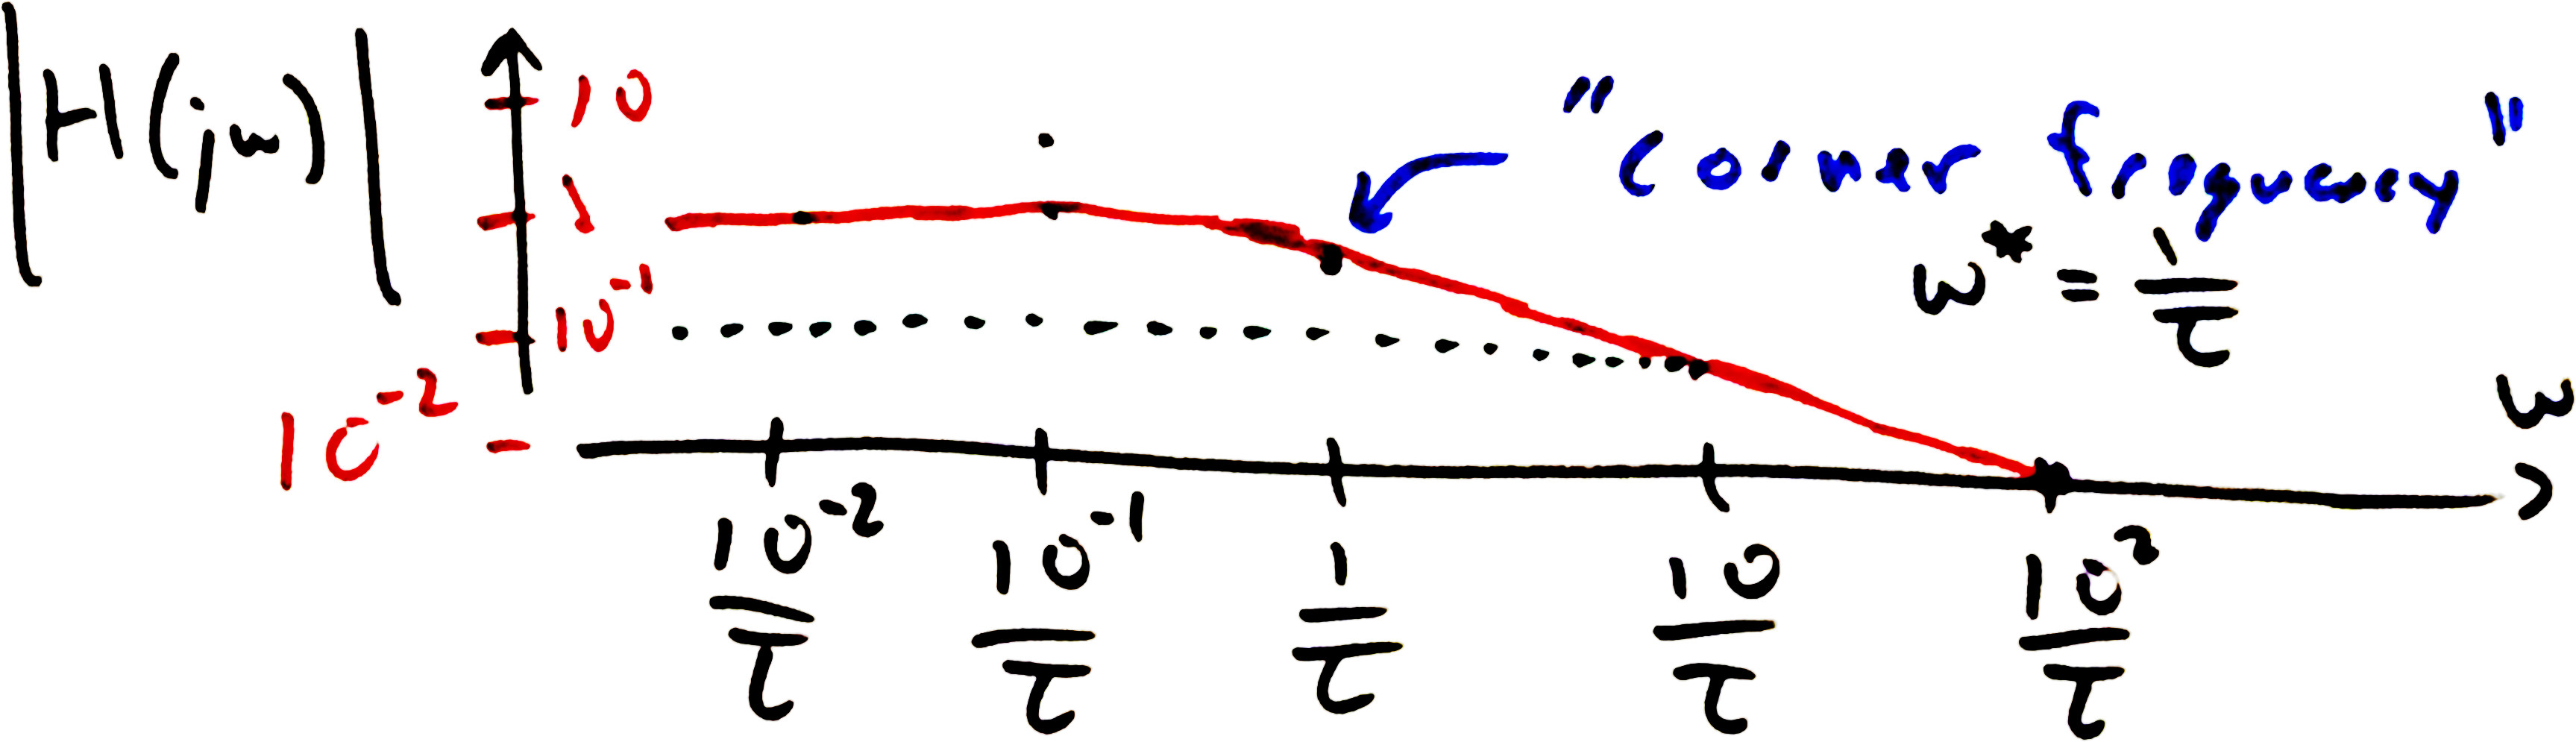
\includegraphics[width=0.7\linewidth]{figures/9/magnitude-bode}
  \caption{Bode magnitude plot of \autoref{eq:lec9-mag-bode}.}
  \label{figure:lec9-mag-bode}
\end{figure}
For \(H(j\omega)\) above,
\begin{align}
  \left|H(j\omega)\right|
  &= \left| \frac{1}{1 + j\omega RC} \right| \\
  &= \frac{1}{\sqrt{1 + \omega^2 (RC)^2}}
\end{align}
On a log-log scale (\autoref{figure:lec9-mag-bode}), this looks approximately like a flat left asymptote and a downhill right asymptote, meeting at \(\eval{H(j\omega)}_{\omega = \frac{1}{\tau}} \approx 1\).\footnote{It's actually \(\frac{1}{\sqrt 2}\) (a real number) but this approximation works better with the piecewise linear style.}

\subsubsection{Phase}
\begin{figure}
  \centering
  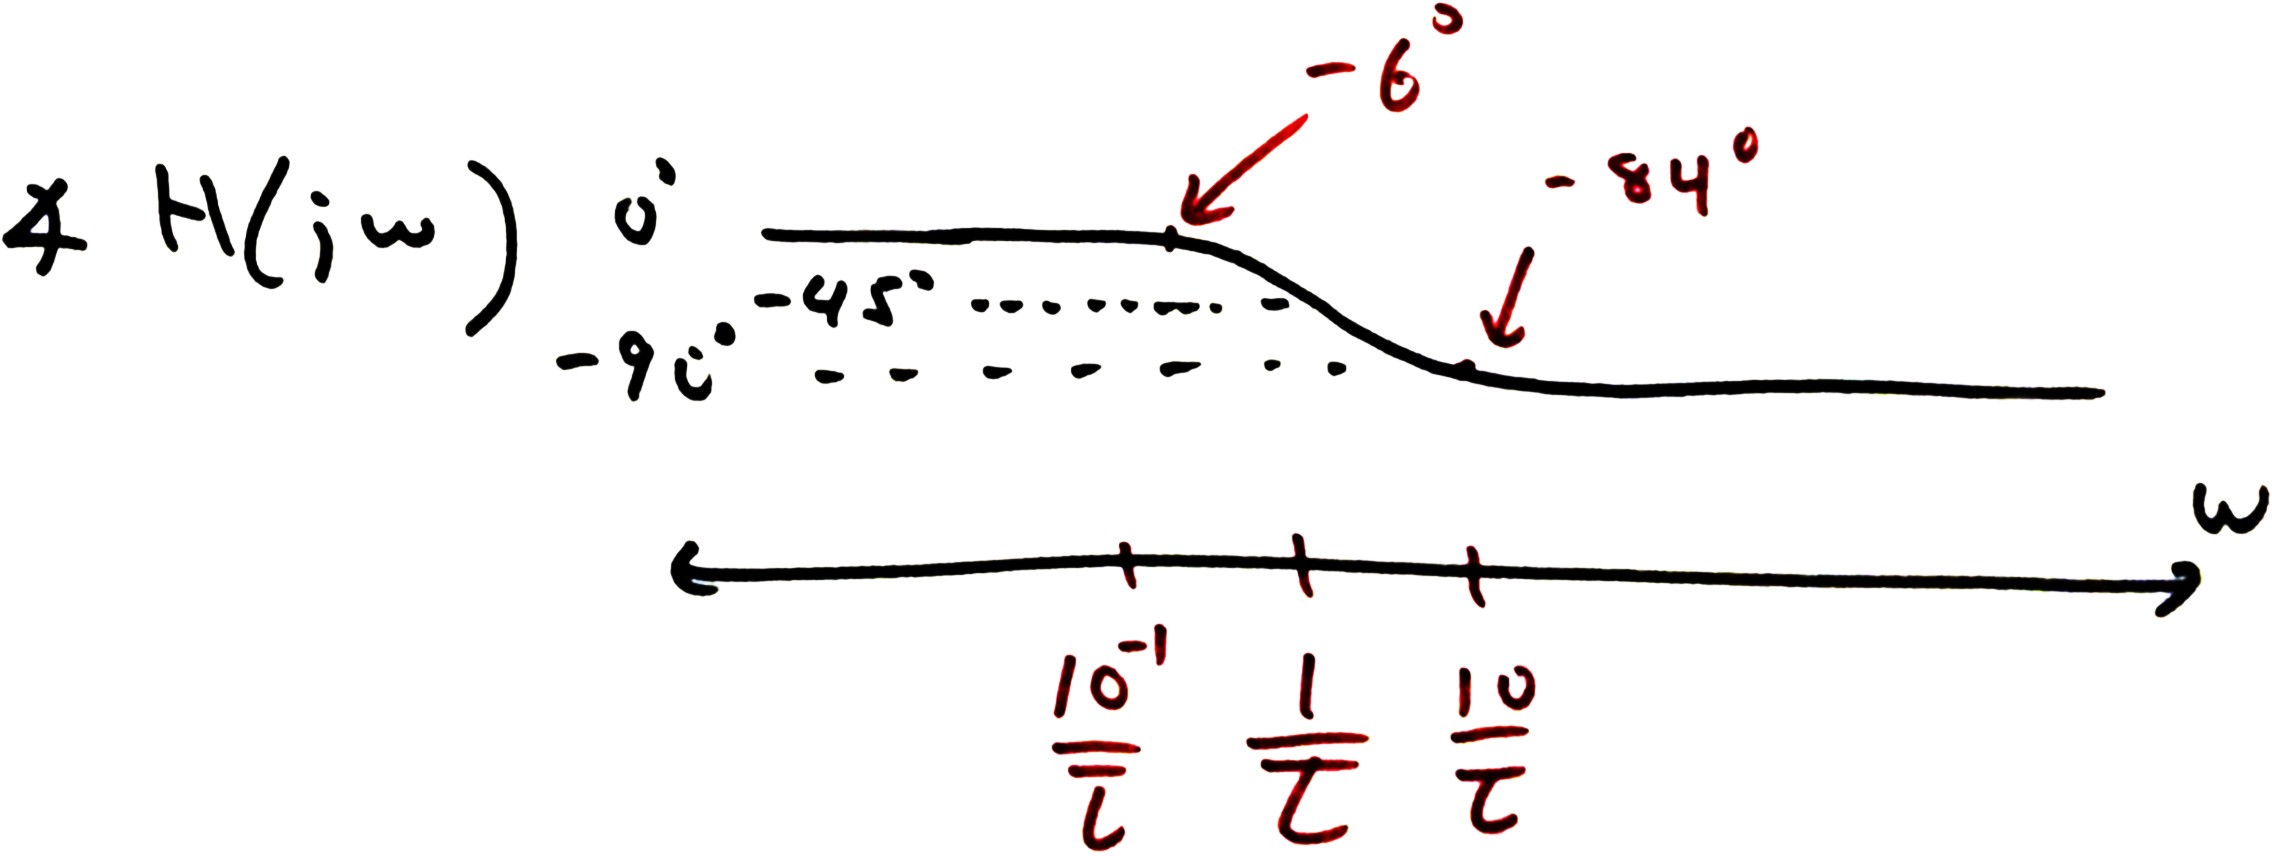
\includegraphics[width=0.7\linewidth]{figures/9/phase-bode}
  \caption{Bode phase plot of \autoref{eq:lec9-mag-bode}.}
  \label{figure:lec9-phase-bode}
\end{figure}
To find the phase of \(H(j\omega)\), we can write it as a complex number in rectangular form, times a real coefficient:
\begin{align}
  H(j\omega) = \frac{1}{1 + j\omega RC}
  &= \frac{1 - j\omega RC}{1 + \omega^2 (RC)^2} = \frac{1 - j\omega \tau}{(\text{\em positive real})}
  \intertext{The numerator is in the fourth quadrant of the complex plane, and its angle of depression is given by}
  \theta &= \tan^{-1} \del{\frac{\text{rise}}{\text{run}}} \\
  &= \tan^{-1} \del{\frac{-\omega \tau}{1}} = \tan^{-1} \del{-\omega \tau}
  \\
  &= -\tan^{-1} \del{\omega \tau}.
\end{align}
For positive inputs on a log scale, the inverse tangent function smoothly transitions from 0 to 90 degrees, crossing 45 degrees at 1.
Our function, plotted in \autoref{figure:lec9-phase-bode}, is the opposite. It has a left asymptote of 0 degrees and a right asyptote of -90 degrees.
The transition, centered at \(\omega^* = \frac{1}{\tau}\), is so fast within a multiple by 10 of \(\omega\) that the asymptotes look nearly flat left and right of the transition region.
